\section{Experiments over 2 axes}
The previous study show the link between the precision and the complexity of the abstraction that we used.
In this part we will use the previous results in order to solve the following problem for different size of the environment:
\begin{figure}
	\center
	\includestandalone[width=0.5\textwidth]{2D_env_problem}
	\caption{Testing environment for the quadricopter.}
	\label{fig:environment}
\end{figure}

\comment{Show the simulation, the runs and so on.}

\subsection{Reduced model $\Ninputs = 1$}
See figure \ref{fig:double_reduce_2D}.

\begin{figure*}
	\center
	\includestandalone[width=\textwidth]{double_reduced_2D}
	\caption{Reduced model with $\Ninputs=1$ in 2D.}
	\label{fig:double_reduce_2D}
\end{figure*}


\subsection{Real case scenarios}
See figure \ref{fig:real_case}.
We have been using the first integrator model in this case (this is the more relevant in the scenario of the wind power).

\begin{figure}[!ht]
  \centering
  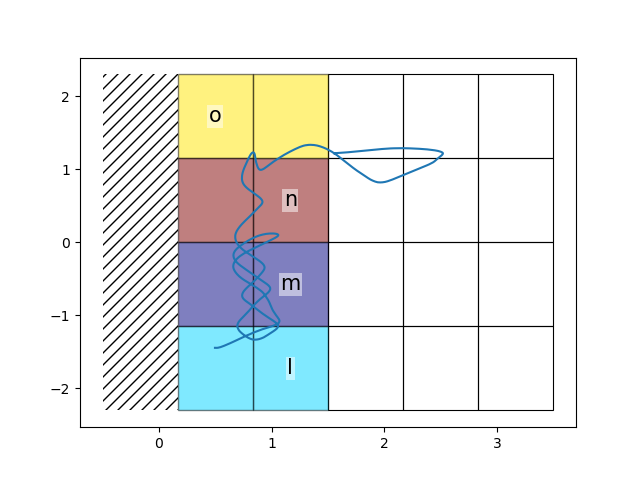
\includegraphics[width=0.9\linewidth]{real_case_scenarios}
  \caption{A trajectory in the state space $(x,v)$.}
  \label{fig:real_case}
\end{figure}

\section{Conclusion}
The strong cyclic planning method can be really effective in some case where the noise.

Conclude about when to use the strongly connected cyclic model.
How to choose the discretization.
Just accept the fact that there is no strong theoretical justifications?
Can I sort of generalize this method to a bigger class of model (not just the first integrator model)?

\comment{I must notice that the we are not using any optimal algorithm (DFS). This imply that the computing time are less than a relevant case scenario.}
